% ============================================================
%  Rolling Horizon Comparison Framework — Oracle Technical Talk
%  Beamer 16:9 · 10pt · v5 (JSON example slides added,
%                             QT4 question reframed)
% ============================================================
\documentclass[aspectratio=169,10pt]{beamer}
\usepackage{tikz}
\usepackage{xcolor}
\usepackage{booktabs}
\usepackage{array}
\usepackage{amsmath}
\usepackage{multirow}
\usepackage[T1]{fontenc}
\usepackage{lmodern}
\usepackage{microtype}
\usepackage{colortbl}
\usetikzlibrary{arrows.meta, shapes.geometric, positioning,
                fit, backgrounds, calc}
% ── COLOURS ──────────────────────────────────────────────────
\definecolor{pblue} {RGB}{0,  60,113}
\definecolor{mblue} {RGB}{0, 100,180}
\definecolor{lblue} {RGB}{200,220,245}
\definecolor{ared}  {RGB}{199, 70, 52}
\definecolor{aorng} {RGB}{215,105, 25}
\definecolor{lgrn}  {RGB}{  0,150, 80}
\definecolor{teal}  {RGB}{  0,130,130}
\definecolor{purp}  {RGB}{120, 50,160}
\definecolor{dgray} {RGB}{ 45, 45, 55}
\definecolor{mgray} {RGB}{130,130,145}
\definecolor{lgray} {RGB}{245,245,248}
% ── THEME ────────────────────────────────────────────────────
\usetheme{default}
\setbeamercolor{frametitle}         {bg=pblue,   fg=white}
\setbeamercolor{structure}          {fg=pblue}
\setbeamercolor{palette primary}    {bg=pblue,   fg=white}
\setbeamercolor{palette secondary}  {bg=mblue,   fg=white}
\setbeamercolor{palette tertiary}   {bg=pblue!70,fg=white}
\setbeamercolor{normal text}        {fg=dgray,   bg=white}
\setbeamercolor{title}              {fg=pblue}
\setbeamercolor{item}               {fg=pblue}
\setbeamercolor{subitem}            {fg=mblue}
\setbeamercolor{block title}        {bg=pblue,   fg=white}
\setbeamercolor{block body}         {bg=lgray,   fg=dgray}
\setbeamercolor{block title alerted}{bg=ared,    fg=white}
\setbeamercolor{block body alerted} {bg=ared!10, fg=dgray}
\setbeamercolor{block title example}{bg=lgrn,    fg=white}
\setbeamercolor{block body example} {bg=lgrn!10, fg=dgray}
\setbeamerfont{frametitle} {series=\bfseries, size=\large}
\setbeamerfont{title}      {series=\bfseries, size=\LARGE}
\setbeamerfont{block title}{series=\bfseries, size=\small}
\setbeamertemplate{navigation symbols}{}
\setbeamertemplate{itemize item}   {\textcolor{pblue}{\small$\blacktriangleright$}}
\setbeamertemplate{itemize subitem}{\textcolor{mblue}{\small$\triangleright$}}
% Frametitle with left colour bar
\setbeamertemplate{frametitle}{%
  \begin{beamercolorbox}[wd=\paperwidth,ht=0.58cm,dp=0.22cm]{frametitle}
    \hspace{0.08cm}%
    \textcolor{aorng}{\rule{0.22cm}{0.42cm}}\hspace{0.22cm}%
    \usebeamerfont{frametitle}\insertframetitle
  \end{beamercolorbox}%
}
% Footer
\setbeamertemplate{footline}{%
  \leavevmode\hbox{%
    \begin{beamercolorbox}[wd=.48\paperwidth,ht=2.2ex,dp=1ex,leftskip=3pt]{palette primary}
      \scriptsize Rolling Horizon Comparison Framework
    \end{beamercolorbox}%
    \begin{beamercolorbox}[wd=.32\paperwidth,ht=2.2ex,dp=1ex,center]{palette secondary}
      \scriptsize Oracle — Technical Presentation
    \end{beamercolorbox}%
    \begin{beamercolorbox}[wd=.20\paperwidth,ht=2.2ex,dp=1ex,right,rightskip=3pt]{palette tertiary}
      \scriptsize \insertframenumber\,/\,\inserttotalframenumber
    \end{beamercolorbox}%
  }%
}
% ── TIKZ STYLES ──────────────────────────────────────────────
\tikzset{
  % Blue agent node
  AB/.style={rectangle,rounded corners=3pt,draw=pblue,fill=pblue!12,
             text width=#1,minimum height=0.55cm,align=center,
             font=\scriptsize,inner sep=3pt,line width=0.65pt},
  AB/.default=2.2cm,
  % Teal tool node
  TB/.style={rectangle,rounded corners=3pt,draw=teal,fill=teal!12,
             text width=#1,minimum height=0.55cm,align=center,
             font=\scriptsize,inner sep=3pt,line width=0.65pt},
  TB/.default=2.0cm,
  % Green data node
  DB/.style={rectangle,rounded corners=3pt,draw=lgrn,fill=lgrn!12,
             text width=#1,minimum height=0.55cm,align=center,
             font=\scriptsize,inner sep=3pt,line width=0.65pt},
  DB/.default=2.0cm,
  % Orange process node
  PB/.style={rectangle,rounded corners=3pt,draw=aorng,fill=aorng!12,
             text width=#1,minimum height=0.55cm,align=center,
             font=\scriptsize,inner sep=3pt,line width=0.65pt},
  PB/.default=2.0cm,
  % Purple cache node
  RB/.style={rectangle,rounded corners=3pt,draw=purp,fill=purp!12,
             text width=#1,minimum height=0.55cm,align=center,
             font=\scriptsize,inner sep=3pt,line width=0.65pt},
  RB/.default=2.0cm,
  % Orange decision diamond
  DC/.style={diamond,draw=aorng,fill=aorng!12,font=\tiny\bfseries,
             align=center,inner sep=1pt,aspect=2.0,
             minimum width=1.4cm,minimum height=0.6cm,line width=0.65pt},
  % Arrows — all clean, no curves
  Arr/.style  ={-{Stealth[length=4pt,width=3pt]},line width=0.8pt,color=pblue},
  GArr/.style ={-{Stealth[length=4pt,width=3pt]},line width=0.8pt,
                color=lgrn,dashed},
  OArr/.style ={-{Stealth[length=4pt,width=3pt]},line width=0.8pt,color=aorng},
}
\title{Rolling Horizon Comparison Framework}
\institute{Oracle}
\date{March 2026}
% ============================================================
\begin{document}
% ============================================================
% ── SLIDE 1 · TITLE (white, clean) ──────────────────────────
\begin{frame}[plain]
  \vspace{1.6cm}
  \begin{center}
    {\color{pblue}\fontsize{24}{28}\selectfont\bfseries
      Rolling Horizon Comparison Framework}
    \par\vspace{10pt}
    \textcolor{pblue!25}{\rule{8cm}{0.6pt}}
    \par\vspace{14pt}
    {\color{mgray}\small
      Oracle \;\textbullet\; 18 March 2026}
  \end{center}
\end{frame}
% ── SLIDE 2 · THE PROBLEM ────────────────────────────────────
\begin{frame}[t]{The Problem — Optimization Models Change Over Time}
\vspace{2pt}
\begin{columns}[T]
  \begin{column}{0.52\textwidth}
    \small
    When an optimization model is updated between planning
    periods, users need answers to four natural questions:
    \vspace{5pt}
    \begin{itemize}\setlength\itemsep{4pt}
      \item \textbf{Structure:} Did the model itself change?
            New constraints, removed variables, shifted parameters?
      \item \textbf{Solution:} How did the optimal decisions shift,
            and by how much?
      \item \textbf{Compatibility:} Can we still execute the previous
            period's plan in the updated model?
      \item \textbf{Attribution:} Why did my solution change?
    \end{itemize}
    \vspace{0pt}
    \begin{alertblock}{Without this framework}
      \small Analysts must manually diff two large Pyomo/Gurobi
      models — slow, error-prone, and inaccessible to non-coders.
    \end{alertblock}
  \end{column}
  \begin{column}{0.44\textwidth}
    \vspace{6pt}
    \begin{center}
    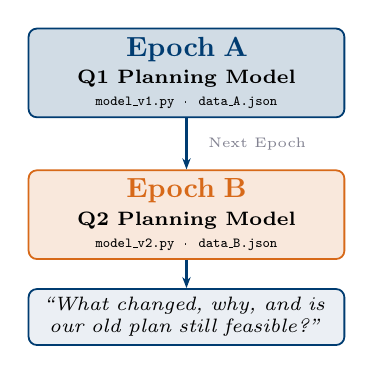
\begin{tikzpicture}
      \node[AB=3.8cm,minimum height=1.1cm,fill=pblue!18,
            font=\scriptsize\bfseries] (A) at (0,3.5)
            {\textcolor{pblue}{\normalsize Epoch A}\\[2pt]
             Q1 Planning Model\\
             \texttt{\tiny model\_v1.py · data\_A.json}};
      \node[PB=3.8cm,minimum height=1.1cm,draw=aorng,fill=aorng!15,
            font=\scriptsize\bfseries] (B) at (0,1.7)
            {\textcolor{aorng}{\normalsize Epoch B}\\[2pt]
             Q2 Planning Model\\
             \texttt{\tiny model\_v2.py · data\_B.json}};
      \draw[Arr,line width=1.2pt] (A.south) -- (B.north)
            node[midway,right=4pt,font=\tiny,text=mgray]{Next Epoch};
      \node[DB=3.8cm,minimum height=0.65cm,draw=pblue,fill=pblue!8,
            font=\scriptsize,align=center] (q) at (0,0.4)
            {\emph{``What changed, why, and is our old plan still feasible?''}};
      \draw[Arr] (B.south) -- (q.north);
    \end{tikzpicture}
    \end{center}
  \end{column}
\end{columns}
\end{frame}
% ── SLIDE 4 · AGENT HIERARCHY ────────────────────────────────
\begin{frame}[t]{Agent Hierarchy}
\vspace{2pt}
\begin{columns}[T]
  \begin{column}{0.67\textwidth}
    \vspace{2pt}
    \begin{center}
    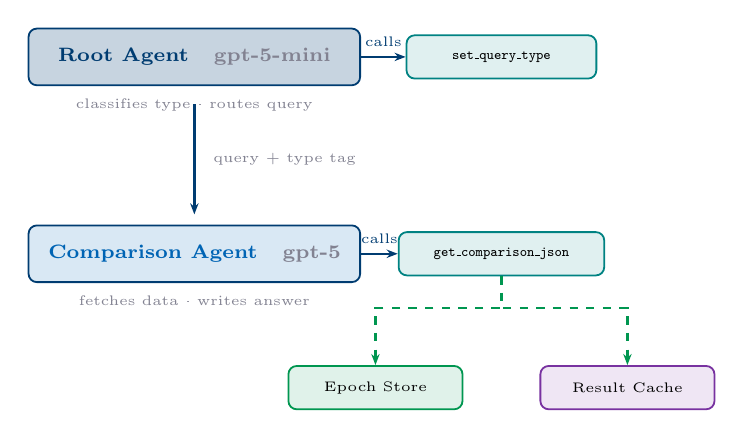
\begin{tikzpicture}
      % Root agent
      \node[AB=4.0cm,fill=pblue!22,minimum height=0.72cm,
            font=\scriptsize\bfseries] at (-1.5,4.6) (root)
            {\textcolor{pblue}{Root Agent}\quad
             \textcolor{mgray}{\scriptsize gpt-5-mini}};
      \node[font=\tiny,text=mgray,below=1pt of root]
            {classifies type · routes query};
      % Root Tool
      \node[TB=2.2cm,font=\tiny] at (2.4, 4.6) (sqt) {\texttt{set\_query\_type}};
      \draw[Arr] (root.east) -- (sqt.west) node[midway,above,font=\tiny]{calls};
      % Arrow Root to Comp
      \draw[Arr,line width=1pt] (-1.5,4.0) -- (-1.5,2.6)
            node[right=3pt,midway,font=\tiny,text=mgray]
            {query + type tag};
      % Comparison agent
      \node[AB=4.0cm,fill=mblue!15,minimum height=0.72cm,
            font=\scriptsize\bfseries] at (-1.5,2.1) (comp)
            {\textcolor{mblue}{Comparison Agent}\quad
             \textcolor{mgray}{\scriptsize gpt-5}};
      \node[font=\tiny,text=mgray,below=1pt of comp]
            {fetches data · writes answer};
      % Comp Tool
      \node[TB=2.4cm,font=\tiny] at (2.4, 2.1) (gcj) {\texttt{get\_comparison\_json}};
      \draw[Arr] (comp.east) -- (gcj.west) node[midway,above,font=\tiny]{calls};
      % Data nodes
      \node[DB=2.0cm,font=\tiny] at (0.8, 0.4) (es) {Epoch Store};
      \node[RB=2.0cm,font=\tiny] at (4.0, 0.4) (rc) {Result Cache};
      \draw[GArr] (gcj.south) -- ++(0,-0.4) -| (es.north);
      \draw[GArr] (gcj.south) -- ++(0,-0.4) -| (rc.north);
    \end{tikzpicture}
    \end{center}
    \vspace{2pt}
    \textcolor{aorng}{\rule[0.4ex]{0.25cm}{0.7pt}}\;
    \textcolor{aorng}{\scriptsize\textit{Prompt rebuilt from scratch before every LLM call — no stale context.}}
  \end{column}
  \begin{column}{0.42\textwidth}
    \begin{block}{Root Agent — the classifier}
      \begin{itemize}\setlength\itemsep{3pt}
        \item Receives the raw natural language question
        \item Passes the category tag + original question
              to the Comparison Agent
      \end{itemize}
    \end{block}
    \begin{block}{Comparison Agent — the analyst}
      \begin{itemize}\setlength\itemsep{3pt}
        \item Uses tools to fetch exactly the
              data it needs
        \item Retrieves a cached QT result or
              triggers the analytics module
        \item Synthesises a natural language answer from data
      \end{itemize}
    \end{block}
  \end{column}
\end{columns}
\end{frame}
% ── SLIDE 3 · SYSTEM ARCHITECTURE ───────────────────────────
\begin{frame}[t]{End-to-End System Architecture}
\vspace{0pt}
\begin{columns}[T]
  % ── Left: layer explanations ──
  \begin{column}{0.45\textwidth}
    \vspace{0pt}
    \begin{block}{\small UI Layer}
      \footnotesize User types in Streamlit; request forwarded
      to the ADK API server via REST
    \end{block}
    \vspace{0pt}
    \begin{block}{\small Agent Layer}
      \footnotesize Root Agent (gpt-5-mini) classifies the query.
      Comparison Agent (gpt-5) calls tools and writes the answer
    \end{block}
    \vspace{0pt}
    \begin{block}{\small Tool Layer}
      \footnotesize \texttt{get\_comparison\_data} checks the
      Result Cache first. On a \textbf{hit} it returns instantly;
      on a \textbf{miss} it delegates to QT modules
    \end{block}
    \vspace{0pt}
    \begin{block}{\small Data Layer}
      \footnotesize QT modules read model artifacts from the
      Epoch Store and \emph{save} answers to the Result Cache
    \end{block}
  \end{column}
  % ── Right: four-layer flow diagram ──
  \begin{column}{0.58\textwidth}
    \vspace{2pt}
    \begin{center}
    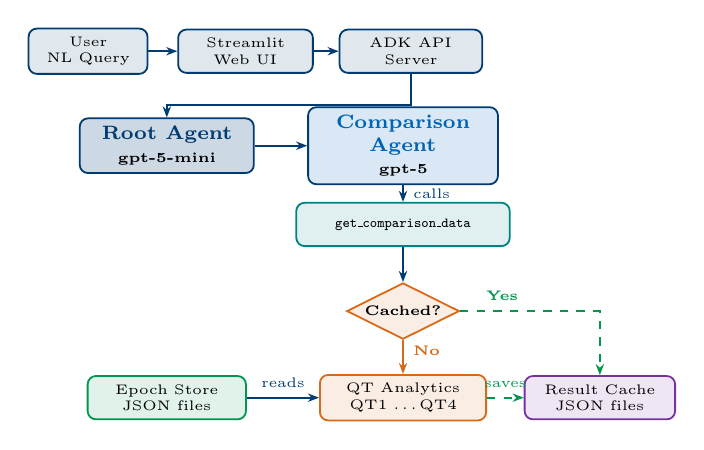
\begin{tikzpicture}
% ── UI layer ─────────────────────────────
\node[AB=1.3cm,font=\tiny] at (0,5.6) (user) {User\\NL Query};
\node[AB=1.5cm,font=\tiny] at (2.0,5.6) (ui) {Streamlit\\Web UI};
\node[AB=1.6cm,font=\tiny] at (4.1,5.6) (api) {ADK API\\Server};
\draw[Arr] (user)--(ui);
\draw[Arr] (ui)--(api);
% ── Agent layer ──────────────────────────
\node[AB=2.0cm,fill=pblue!20,font=\scriptsize\bfseries]
at (1.0,4.4) (root)
{\textcolor{pblue}{Root Agent}\\{\tiny gpt-5-mini}};
\node[AB=2.2cm,fill=mblue!15,font=\scriptsize\bfseries]
at (4.0,4.4) (comp)
{\textcolor{mblue}{Comparison Agent}\\{\tiny gpt-5}};
\draw[Arr] (api.south) -- ++(0,-0.4) -| (root.north);
\draw[Arr] (root.east) -- (comp.west);
% ── Tool layer ───────────────────────────
\node[TB=2.5cm,font=\tiny] at (4.0, 3.4) (tools)
{\texttt{get\_comparison\_data}};
\node[DC] at (4.0, 2.3) (chk) {Cached?};
\draw[Arr] (comp.south) -- (tools.north) node[midway,right,font=\tiny]{calls};
\draw[Arr] (tools.south) -- (chk.north);
% ── Data layer ───────────────────────────
\node[DB=1.8cm,font=\tiny] at (1.0, 1.2) (epoch) {Epoch Store\\JSON files};
\node[PB=1.9cm,font=\tiny] at (4.0, 1.2) (qt)    {QT Analytics\\QT1 \dots QT4};
\node[RB=1.7cm,font=\tiny] at (6.5, 1.2) (cache) {Result Cache\\JSON files};
% Cache hit logic
\draw[GArr] (chk.east) -| node[pos=0.15,above,font=\tiny]{\textbf{Yes}} (cache.north);
\draw[OArr] (chk.south) -- node[pos=0.3,right,font=\tiny]{\textbf{No}} (qt.north);
% Data operations
\draw[Arr] (epoch.east) -- (qt.west) node[midway,above,font=\tiny]{reads};
\draw[GArr] (qt.east) -- (cache.west) node[midway,above,font=\tiny]{saves};
\end{tikzpicture}
    \end{center}
  \end{column}
\end{columns}
\end{frame}
% ── SLIDE 5 · QUERY CLASSIFICATION ──────────────────────────
\begin{frame}[t]{Query Classification — The Root Agent Decides}
\vspace{2pt}
\begin{columns}[T]
  \begin{column}{0.46\textwidth}
    \vspace{2pt}
    \begin{center}
      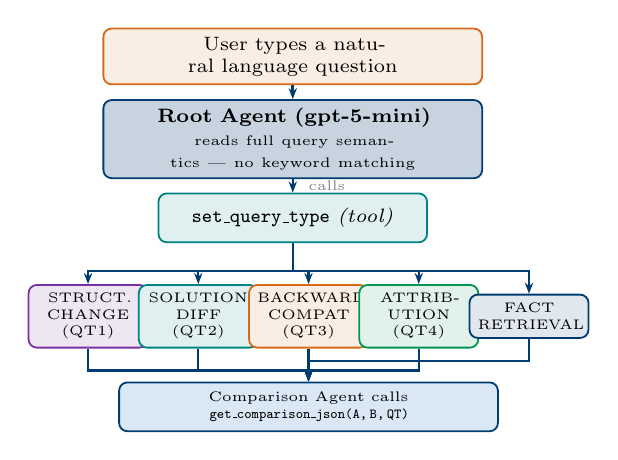
\begin{tikzpicture}
        % User question
        \node[PB=4.6cm,minimum height=0.6cm,font=\scriptsize]
              at (0,5.2) (q)
              {User types a natural language question};
        % Root Agent
        \node[AB=4.6cm,fill=pblue!22,minimum height=0.85cm,
              font=\scriptsize] at (0,4.15) (ra)
              {\textbf{Root Agent (gpt-5-mini)}\\
               {\tiny reads full query semantics — no keyword matching}};
        \draw[Arr,line width=1pt] (q)--(ra);
        % set_query_type tool (Root Agent calls this)
        \node[TB=3.2cm,minimum height=0.62cm,font=\scriptsize]
              at (0,3.15) (sqt)
              {\texttt{set\_query\_type} \textit{(tool)}};
        \draw[Arr] (ra.south) -- (sqt.north)
              node[midway,right=2pt,font=\tiny,text=mgray]{calls};
        % Five tag output boxes — fan-out from set_query_type
        \node[RB=1.3cm,font=\tiny] at (-2.6,1.9) (c1)
              {STRUCT.\\CHANGE\\(QT1)};
        \node[TB=1.3cm,font=\tiny]  at (-1.2,1.9) (c2)
              {SOLUTION\\DIFF\\(QT2)};
        \node[PB=1.3cm,font=\tiny]  at ( 0.2,1.9) (c3)
              {BACKWARD\\COMPAT\\(QT3)};
        \node[DB=1.3cm,font=\tiny]  at ( 1.6,1.9) (c4)
              {ATTRIB-\\UTION\\(QT4)};
        \node[AB=1.3cm,font=\tiny]  at ( 3.0,1.9) (c5)
              {FACT\\RETRIEVAL};
        \foreach \c in {c1,c2,c3,c4,c5}
          \draw[Arr] (sqt.south) -- ++(0,-0.35) -| (\c.north);
        % All tags converge → get_comparison_json
        \node[AB=4.6cm,fill=mblue!15,minimum height=0.62cm,
              font=\tiny] at (0.2,0.75) (gc)
              {Comparison Agent calls
               \texttt{get\_comparison\_json(A,\,B,\,QT)}};
        \foreach \c in {c1,c2,c3,c4,c5}
          \draw[Arr] (\c.south) -- ++(0,-0.28) -| (gc.north);
        % Broad vs narrow note
      \end{tikzpicture}
    \end{center}
  \end{column}
  \begin{column}{0.50\textwidth}
    \vspace{4pt}
    \begin{exampleblock}{Why use an LLM to classify?}
      \small Questions are inherently ambiguous:
      \vspace{3pt}
      \begin{itemize}\setlength\itemsep{4pt}
        \item \emph{``Is our old plan still valid?''}\\
              \textcolor{aorng}{$\to$ QT3 (backward compat.),}\\
        \item \emph{``Why did Chicago's quota drop?''}\\
              \textcolor{aorng}{$\to$ QT4 (attribution),}\\
        \item \emph{``Did we add any new routes?''}\\
              \textcolor{aorng}{$\to$ QT1 (structural),}\\
      \end{itemize}
    \end{exampleblock}
    \vspace{5pt}
  \end{column}
\end{columns}
\end{frame}
% ── SLIDE 6 · NL → VARIABLE RESOLUTION ──────────────────────
\begin{frame}[t]{How the System Knows Which Variable You Mean}
\vspace{2pt}
\begin{columns}[T]
  \begin{column}{0.44\textwidth}
    \vspace{2pt}
    \begin{center}
    \begin{tikzpicture}
      \node[PB=4.3cm,minimum height=0.55cm,font=\scriptsize]
            at (0,5.6) (q)
            {\emph{``demand for Chicago''} (user's words)};
      \node[TB=4.3cm,minimum height=0.55cm,font=\scriptsize]
            at (0,4.75) (f1)
            {\texttt{get\_epoch\_data(hint=''demand chicago'')}};
      \draw[Arr] (q)--(f1);
      \node[DB=4.3cm,minimum height=0.65cm,font=\tiny]
            at (0,3.85) (fl)
            {Returns full family list:\\
             \texttt{[demand, supply, cost, assign, route, ...]}\strut};
      \draw[Arr] (f1)--(fl);
      \node[font=\tiny,text=aorng,align=center]
            at (0,3.35) {\textit{Always small — tens of names, never thousands}};
      \node[AB=4.3cm,minimum height=0.55cm,font=\scriptsize]
            at (0,2.75) (llm)
            {LLM maps phrase $\to$ family \texttt{"demand"}};
      \draw[Arr] (fl)--(llm);
      \node[TB=4.3cm,minimum height=0.55cm,font=\scriptsize]
            at (0,1.90) (f2)
            {\texttt{get\_epoch\_data(family=''demand'')}};
      \draw[Arr] (llm)--(f2);
      \node[DB=4.3cm,minimum height=0.75cm,font=\tiny]
            at (0,0.95) (out)
            {\texttt{demand[Chicago]}: A=142 · B=168\\
             \texttt{demand[Houston]}: A=98 · B=91\ \ldots};
      \draw[Arr] (f2)--(out);
    \end{tikzpicture}
    \end{center}
  \end{column}
  \begin{column}{0.6\textwidth}
    \vspace{4pt}
    \small\textbf{The challenge:} A user says
    \emph{``demand for Chicago''}.
    The model variable might be \texttt{demand},
    \texttt{d}, \texttt{dem\_node}, or \texttt{flow\_in}
 , depending on the modeler's naming convention.
    \vspace{8pt}
    \begin{block}{Two-step resolution strategy}
      \begin{itemize}\setlength\itemsep{5pt}
        \item \textbf{Step 1 — discover:} Fetch the complete list
              of family names from the epoch store.
              This is always small (tens of names).
        \item \textbf{Step 2 — match:} The LLM compares the user's
              phrase to those names semantically.
              \emph{``demand''} correctly matches
              \texttt{dem\_node} even without an exact string match.
        \item \textbf{Step 3 — fetch:} Retrieve values for that
              specific family only.
              Capped at \textbf{200 entries} to stay within
              the context budget.
      \end{itemize}
    \end{block}
  \end{column}
\end{columns}
\end{frame}
% ── SLIDE 7 · PROMPT CONSTRUCTION ───────────────────────────
\begin{frame}[t]{How the Prompt Is Built Before Every LLM Call}
\vspace{2pt}
\begin{columns}[T]
  \begin{column}{0.50\textwidth}
    \vspace{2pt}
    \begin{center}
    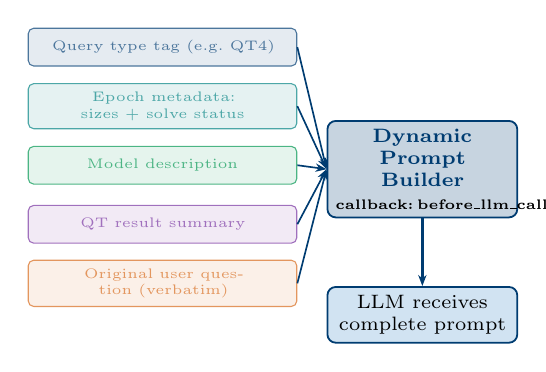
\begin{tikzpicture}
      % Five input boxes — left column at x = -1.5
      \node[pblue!70,rectangle,rounded corners=2pt,draw,fill=pblue!10,
            font=\tiny,inner sep=3pt,text width=3.2cm,
            minimum height=0.48cm,align=center]
            at (-1.5,5.2) (i1) {Query type tag (e.g.\ QT4)};
      \node[teal!70,rectangle,rounded corners=2pt,draw,fill=teal!10,
            font=\tiny,inner sep=3pt,text width=3.2cm,
            minimum height=0.48cm,align=center]
            at (-1.5,4.45) (i2) {Epoch metadata: sizes + solve status};
      \node[lgrn!70,rectangle,rounded corners=2pt,draw,fill=lgrn!10,
            font=\tiny,inner sep=3pt,text width=3.2cm,
            minimum height=0.48cm,align=center]
            at (-1.5,3.7) (i3) {Model description};
      \node[purp!70,rectangle,rounded corners=2pt,draw,fill=purp!10,
            font=\tiny,inner sep=3pt,text width=3.2cm,
            minimum height=0.48cm,align=center]
            at (-1.5,2.95) (i4) {QT result summary};
      \node[aorng!70,rectangle,rounded corners=2pt,draw,fill=aorng!10,
            font=\tiny,inner sep=3pt,text width=3.2cm,
            minimum height=0.48cm,align=center]
            at (-1.5,2.2) (i5) {Original user question (verbatim)};
      % Builder node — right side, vertically centred
      \node[AB=2.2cm,fill=pblue!22,minimum height=1.1cm,
            font=\scriptsize\bfseries]
            at (1.8,3.65) (build)
            {\textcolor{pblue}{Dynamic\\Prompt Builder}\\
             {\tiny callback:\,before\_llm\_call}};
      % Arrows — all horizontal to builder
      \foreach \i in {i1,i2,i3,i4,i5}
        \draw[Arr,line width=0.6pt] (\i.east) -- (build.west);
      % Output
      \node[AB=2.2cm,fill=mblue!18,minimum height=0.6cm,font=\scriptsize]
            at (1.8,1.8) (llm)
            {LLM receives\\complete prompt};
      \draw[Arr,line width=1pt] (build.south) -- (llm.north);
    \end{tikzpicture}
    \end{center}
    \vspace{2pt}
    \textcolor{aorng}{\rule[0.4ex]{0.25cm}{0.7pt}}\;
    \textcolor{aorng}{\scriptsize\textit{Rebuilt fresh before every single LLM call — never reused.}}
  \end{column}
  \begin{column}{0.55\textwidth}
    \vspace{4pt}
    \begin{block}{Why rebuild every time?}
      \small Between two conversation turns, the session
      state can change: a QT result may have just been
      cached, or the user asked a follow-up requiring
      different family data. Rebuilding guarantees the
      LLM always has accurate, up-to-date context.
    \end{block}
  \end{column}
\end{columns}
\end{frame}
% ── SLIDE 9 · EPOCH DATA STORE ──────────────────────────────
\begin{frame}[t]{Epoch Data Store}
\vspace{2pt}
\begin{columns}[T]
  \begin{column}{0.47\textwidth}
    \textbf{Per-epoch files (written once at registration):}
    \vspace{4pt}
    \renewcommand{\arraystretch}{1.25}
    \begin{tabular}{@{}p{2.5cm} p{3.5cm}@{}}
      \texttt{model.pkl}      & Cloudpickle of solved Pyomo model \\
      \texttt{solution.json}  & Objective + all variable values \\
      \texttt{params.json}    & All parameter families + values \\
      \texttt{structure.json} & Index sets, var/con families \\
      \texttt{meta.json}      & $n_{\text{vars}}$, $n_{\text{cons}}$, status \\
      \texttt{duals.json}     & Shadow prices — computed on first QT4 call only \\
    \end{tabular}
  \end{column}
  \begin{column}{0.49\textwidth}
    \begin{center}
    \begin{tikzpicture}
      \node[DB=5.5cm,minimum height=0.6cm,fill=lgrn!22,
            font=\scriptsize\bfseries] at (0,4.5) (reg)
            {\texttt{tmp/rh\_epochs/registry.json}};
      \node[font=\tiny,text=mgray,align=center] at (0,4.05)
            {global index of all registered epochs};
      \node[AB=2.3cm,font=\scriptsize] at (-1.45,3.1) (ea)
            {\texttt{epoch\_id\_A/}};
      \node[AB=2.3cm,font=\scriptsize] at ( 1.45,3.1) (eb)
            {\texttt{epoch\_id\_B/}};
      \draw[Arr] (reg.south) -- ++(0,-0.35) -| (ea.north);
      \draw[Arr] (reg.south) -- ++(0,-0.35) -| (eb.north);
      \node[TB=2.1cm,minimum height=0.85cm,font=\tiny] at (-1.45,1.8) (fa)
            {model.pkl\\solution.json\\params.json \ldots};
      \node[TB=2.1cm,minimum height=0.85cm,font=\tiny] at ( 1.45,1.8) (fb)
            {model.pkl\\solution.json\\params.json \ldots};
      \draw[GArr] (ea)--(fa);
      \draw[GArr] (eb)--(fb);
      \node[RB=5.0cm,minimum height=0.7cm,font=\tiny] at (0,0.55) (cmp)
            {comparisons/\{A\}\_vs\_\{B\}/\\
             qt1 · qt2 · qt3 · qt4\texttt{.json}};
      \draw[GArr] (fa.south) -- ++(0,-0.25) -| (cmp.west);
      \draw[GArr] (fb.south) -- ++(0,-0.25) -| (cmp.east);
    \end{tikzpicture}
    \end{center}
    \vspace{2pt}
    \textcolor{aorng}{\rule[0.4ex]{0.25cm}{0.7pt}}\;
    \textcolor{aorng}{\scriptsize\textit{\texttt{duals.json} is the only file not written at registration — it needs a solver call and is generated lazily on first QT4 query.}}
  \end{column}
\end{columns}
\end{frame}
% ── SLIDE 10 · CORE DATA STRUCTURES ─────────────────────────
\begin{frame}[t]{Core Data Structures}
\vspace{2pt}
\begin{columns}[T]
  \begin{column}{0.48\textwidth}
    \begin{block}{\texttt{EpochMeta} — registry entry per epoch}
      \texttt{\scriptsize
        \{\,"epoch\_id": "q1\_plan\_abc1",\\
        \quad "label": "Q1 Supply Chain",\\
        \quad "n\_vars": 1240,\ "n\_cons": 840,\\
        \quad "solve\_status": "optimal",\\
        \quad "obj\_value": 482310.5,\\
        \quad "var\_families": ["demand","assign",...],\\
        \quad "param\_families": ["cost","cap",...]\,\}
      }
    \end{block}
    \vspace{5pt}
    \begin{block}{\texttt{solution.json} — per epoch}
      \texttt{\scriptsize
        \{\,"objective": 482310.5,\\
        \quad "variables":\,\{\\
        \qquad "assign[Chi]":\,\{"value":142,"dual":0\},\\
        \qquad ...\,\},\\
        \quad "constraints":\,\{\\
        \qquad "cap[Chi]":\,\{"slack":0,"dual":2.1\},\\
        \qquad ...\,\}\,\}
      }
    \end{block}
  \end{column}
  \begin{column}{0.48\textwidth}
    \begin{block}{Uniform QT result schema (all four modules)}
      \texttt{\scriptsize
        \{\,"qt": "QT2",\\
        \quad "epoch\_a": "q1\_plan\_abc1",\\
        \quad "epoch\_b": "q2\_plan\_def2",\\
        \quad "summary":\,\{...\},\ \textcolor{mgray}{// key metrics}\\
        \quad "items":\,[...],\ \textcolor{mgray}{\ \ \ // capped list}\\
        \quad "truncated": true,\\
        \quad "total\_count": 348\,\}
      }
    \end{block}
    \vspace{5pt}
    \begin{alertblock}{One schema for all four modules}
      \small Every QT module returns the same outer structure.
      The Comparison Agent always knows how to navigate any
      result — even for a module it has not seen before.
      The inner \texttt{summary} and \texttt{items} fields
      are QT-specific.
    \end{alertblock}
  \end{column}
\end{columns}
\end{frame}

% ── TRUNCATION — PART 1: WHAT IT IS ─────────────────────────
\begin{frame}[t]{Token Caps — Every Tool Response Has a Hard Limit}
\vspace{2pt}
\begin{columns}[T]
  \begin{column}{0.48\textwidth}
    \vspace{4pt}
    \begin{alertblock}{The problem}
      \small A single model can have thousands of variables and
      parameters. Returning everything in one tool call would
      overflow the LLM's context window instantly.
    \end{alertblock}
    \vspace{6pt}
    \begin{block}{Hard caps per call}
      \renewcommand{\arraystretch}{1.4}
      \small
      \begin{tabular}{@{}p{5.2cm}r@{}}
        \toprule
        \textbf{Call type} & \textbf{Max} \\
        \midrule
        QT result \texttt{items} (any QT)  & 20  \\
        \texttt{variable\_family} drill-down & 200 \\
        \texttt{param\_family} drill-down    & 200 \\
        Bulk variable / param list          & 100 \\
        Index sets                          & 30  \\
        \bottomrule
      \end{tabular}
    \end{block}
    \vspace{6pt}
    \begin{block}{Two fields always present when capped}
      \begin{itemize}\setlength\itemsep{4pt}
        \item \texttt{"truncated": true} \textcolor{mgray}{—} explicit signal
        \item \texttt{"total\_count": N} \textcolor{mgray}{—} how many exist in total
      \end{itemize}
    \end{block}
  \end{column}
  \begin{column}{0.48\textwidth}
    \vspace{4pt}
    \begin{block}{What a capped QT2 response looks like}
      \texttt{\scriptsize
        \{\\
        \quad "qt": "QT2",\\
        \quad "summary": \{"obj\_delta": ...\},\\[3pt]
        \quad "items": [\hfill\textcolor{teal}{\tiny only top 20 of 246 arrive}\\
        \quad\quad \{"variable": "assign[Chi]", ...\},\\
        \quad\quad \{"variable": "assign[Hou]", ...\},\\
        \quad\quad \ldots\ \textcolor{mgray}{// 18 more}\\
        \quad ],\\[5pt]
        \quad \textcolor{ared}{\bfseries "truncated": true,}\hfill\textcolor{ared}{\tiny agent reads this flag}\\
        \quad \textcolor{ared}{\bfseries "total\_count": 246}\hfill\textcolor{ared}{\tiny 226 entries not visible}\\
        \}
      }
    \end{block}
    \vspace{5pt}
    \textcolor{aorng}{\rule[0.4ex]{0.25cm}{0.7pt}}\;
    \textcolor{aorng}{\scriptsize\textit{The agent treats \texttt{truncated: true} as a signal
    to make a targeted follow-up call — never guesses from partial data.}}
  \end{column}
\end{columns}
\end{frame}

% ── TRUNCATION — PART 2: HOW THE AGENT DRILLS DOWN ───────────
\begin{frame}[t]{Progressive Disclosure — The Agent Drills Down}
\vspace{2pt}
\begin{columns}[T]
  \begin{column}{0.44\textwidth}
    \vspace{2pt}
    \begin{center}
    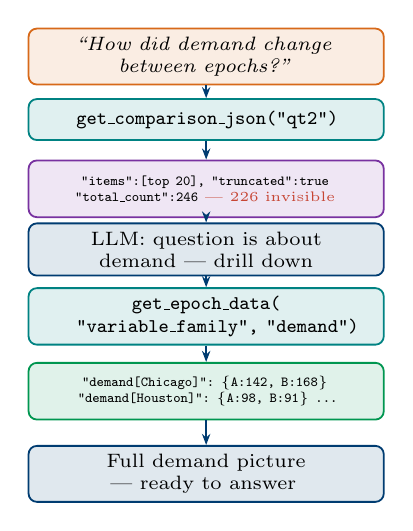
\begin{tikzpicture}
      \node[PB=4.3cm,minimum height=0.52cm,font=\scriptsize]
            at (0,5.5) (q)
            {\emph{``How did demand change between epochs?''}};
      \node[TB=4.3cm,minimum height=0.52cm,font=\scriptsize]
            at (0,4.7) (c1)
            {\texttt{get\_comparison\_json("qt2")}};
      \draw[Arr] (q)--(c1);
      \node[RB=4.3cm,minimum height=0.72cm,font=\tiny,align=center]
            at (0,3.82) (r1)
            {\texttt{"items":[top 20],\ "truncated":true}\\
             \texttt{"total\_count":246}\ \textcolor{ared}{\tiny — 226 invisible}};
      \draw[Arr] (c1)--(r1);
      \node[AB=4.3cm,minimum height=0.52cm,font=\scriptsize]
            at (0,3.05) (dec)
            {LLM: question is about demand — drill down};
      \draw[Arr] (r1)--(dec);
      \node[TB=4.3cm,minimum height=0.60cm,font=\scriptsize]
            at (0,2.2) (c2)
            {\texttt{get\_epoch\_data(}\\
             \texttt{\quad"variable\_family",\ "demand")}};
      \draw[Arr] (dec)--(c2);
      \node[DB=4.3cm,minimum height=0.72cm,font=\tiny,align=center]
            at (0,1.25) (r2)
            {\texttt{"demand[Chicago]":\ \{A:142,\ B:168\}}\\
             \texttt{"demand[Houston]":\ \{A:98,\ B:91\}\ \ldots}};
      \draw[Arr] (c2)--(r2);
      \node[AB=4.3cm,minimum height=0.48cm,font=\scriptsize]
            at (0,0.2) (ans)
            {Full demand picture — ready to answer};
      \draw[Arr] (r2)--(ans);
    \end{tikzpicture}
    \end{center}
  \end{column}
  \begin{column}{0.65\textwidth}
    \vspace{4pt}
    \small\textbf{Step by step:}
    \begin{enumerate}\setlength\itemsep{2pt}
      \item \textbf{First call:} Agent calls
            \texttt{get\_comparison\_json("qt2")} for the
            solution diff summary.
      \item \textbf{Truncated result:} Only top 20 variable
            changes arrive. Agent sees \texttt{"truncated": true}
            and \texttt{"total\_count": 246} — knows 226 changes
            are invisible.
      \item \textbf{Decision:} Question is about demand
            specifically. No need to see all 246 changes —
            only the demand family matters.
      \item \textbf{Targeted drill-down:} Agent calls
            \texttt{get\_epoch\_data("variable\_family","demand")}.
            Returns up to 200 entries for \emph{demand only}
            across both epochs.
      \item \textbf{Answer:} Agent has all demand values for
            Epoch A and B. Gives a complete, accurate answer
            without ever fetching all 246 changes.
    \end{enumerate}
    \vspace{6pt}
    \textcolor{aorng}{\rule[0.4ex]{0.25cm}{0.7pt}}\;
    \textcolor{aorng}{\scriptsize\textit{Start broad, drill where needed — never dump everything at once.}}
  \end{column}
\end{columns}
\end{frame}

% ── SLIDE 12 · QT1 ───────────────────────────────────────────
\begin{frame}[t]{QT1 — Structural Diff: What Changed in the Model Itself?}
\vspace{2pt}
\begin{columns}[T]
  \begin{column}{0.52\textwidth}
    \small\textbf{User asks:}
    \emph{``Did new constraints get added? Which parameters shifted most?''}
    \vspace{5pt}
    \textbf{Algorithm — pure Python, zero solver calls:}
    \begin{enumerate}\setlength\itemsep{3pt}
      \item Load \texttt{structure.json} from both epochs
            (no model unpickling needed)
      \item Compare \textbf{index sets}: elements added / removed
      \item Compare \textbf{variable families}: new or dropped families
      \item Compare \textbf{constraint templates}: new or dropped rules
      \item For each \texttt{(family, index)} parameter pair, compute
            relative shift $\delta = (p_B - p_A)\,/\,|p_A|$
      \item Classify magnitude:\\
            \textcolor{lgrn}{\textbf{SMALL}} $|\delta|{<}10\%$\quad
            \textcolor{aorng}{\textbf{MOD.}} $10{-}30\%$\quad
            \textcolor{ared}{\textbf{LARGE}} ${\geq}30\%$
    \end{enumerate}
  \end{column}
  \begin{column}{0.56\textwidth}
    \begin{block}{Input data structures}
      \begin{itemize}\setlength\itemsep{1pt}
        \item \texttt{structure.json}:\\
              \texttt{\small \{index\_sets, var\_families,}\\
              \texttt{\small \phantom{x}con\_templates, params\}}
        \item Both epochs needed; no raw Pyomo model
        \item Numerical noise filter: shifts $<\!10^{-6}$ ignored
      \end{itemize}
    \end{block}
    \vspace{5pt}
    \begin{block}{Output JSON (QT1 result)}
      \begin{itemize}\setlength\itemsep{1pt}
        \item \texttt{added\_var\_families}: new families
        \item \texttt{removed\_var\_families}: dropped families
        \item \texttt{set\_changes}: per-set added/removed elements
        \item \texttt{param\_changes}: top 20 sorted by $|\delta|$,
              each tagged SMALL / MOD / LARGE
      \end{itemize}
    \end{block}
    \vspace{4pt}
  \end{column}
\end{columns}
\end{frame}

% ── QT1 JSON EXAMPLE ─────────────────────────────────────────
\begin{frame}[t]{QT1 JSON — \texttt{get\_comparison\_json("qt1")} Return Value}
\vspace{1pt}
\begin{block}{}
  \texttt{\scriptsize
    \{\,"qt": "QT1",\\
    \quad "epoch\_a": "q1\_supply\_abc",\\
    \quad "epoch\_b": "q2\_supply\_def",\\[1pt]
    \quad "summary": \{\hfill\textcolor{pblue}{\tiny structural facts — always complete, never capped}\\
    \quad\quad "added\_var\_families": ["emergency\_supply"],\hfill\textcolor{aorng}{\tiny family exists in B but not A}\\
    \quad\quad "removed\_var\_families": [],\hfill\textcolor{mgray}{\tiny nothing dropped}\\
    \quad\quad "set\_changes": \{\\
    \quad\quad\quad "NODES": \{\\
    \quad\quad\quad\quad "added": ["Denver"],\hfill\textcolor{aorng}{\tiny new index element in Epoch B}\\
    \quad\quad\quad\quad "removed": []\hfill\textcolor{mgray}{\tiny no elements disappeared}\\
    \quad\quad\quad \}\\
    \quad\quad \}\\
    \quad \},\\[1pt]
    \quad "items": [\hfill\textcolor{teal}{\tiny parameter shifts — ranked by $|\delta|$, capped at 20}\\
    \quad\quad \{\\
    \quad\quad\quad "family": "demand",\hfill\textcolor{mgray}{\tiny which parameter family}\\
    \quad\quad\quad "index":\ "Chicago",\hfill\textcolor{mgray}{\tiny which index element}\\
    \quad\quad\quad "delta":\ 0.185,\hfill\textcolor{pblue}{\tiny $(p_B - p_A)/|p_A|$ = +18.5\%}\\
    \quad\quad\quad "magnitude": "MOD"\hfill\textcolor{aorng}{\tiny $<$10\% \textrm{SMALL}\;|\;10-30\% \textrm{MOD}\;|\;$\geq$30\% \textrm{LARGE}}\\
    \quad\quad \},\\
    \quad\quad \ldots\quad\textcolor{mgray}{// 87 parameter shifts total}\\
    \quad ],\\
    \quad "truncated": true,\hfill\textcolor{ared}{\tiny list was cut — not all items shown}\\
    \quad "total\_count": 87\hfill\textcolor{ared}{\tiny only 20 of 87 shown — 67 invisible to agent}\\
    \}
  }
\end{block}
\vspace{1pt}
\centering\scriptsize
\textcolor{pblue}{$\blacksquare$}\,Computed metric\quad
\textcolor{aorng}{$\blacksquare$}\,Structural change\quad
\textcolor{ared}{$\blacksquare$}\,High-magnitude / truncation\quad
\textcolor{mgray}{$\blacksquare$}\,Metadata\qquad
\textcolor{mgray}{\textit{Pure structure comparison — no solver calls needed.}}
\end{frame}

% ── SLIDE 13 · QT2 ───────────────────────────────────────────
\begin{frame}[t]{QT2 — Solution Diff: How Did the Optimal Solution Change?}
\vspace{2pt}
\begin{columns}[T]
  \begin{column}{0.50\textwidth}
    \small\textbf{User asks:}
    \emph{``Did costs go up? Which decisions changed most? Did any binary decisions flip?''}
    \vspace{5pt}
    \textbf{Algorithm — pure Python, zero solver calls:}
    \begin{enumerate}\setlength\itemsep{3pt}
      \item Load \texttt{solution.json} from both epochs
      \item Compute \textbf{objective gap}:
            $\Delta_{\text{obj}} = \text{obj}_B - \text{obj}_A$
      \item For each variable, compute
            $\delta_i = (v_i^B - v_i^A)\,/\,|v_i^A|$;
            flag if $|\delta_i| > 10^{-5}$
      \item Compute \textbf{churn rate}: fraction of
            variables that changed
      \item Track \textbf{binary activations} (0$\to$1)
            and \textbf{deactivations} (1$\to$0)
      \item Compare \textbf{binding status} of constraints
    \end{enumerate}
  \end{column}
  \begin{column}{0.55\textwidth}
    \begin{block}{Key metrics in the QT2 output}
      \begin{itemize}\setlength\itemsep{3pt}
        \item \texttt{obj\_delta}: absolute + relative gap
        \item \texttt{churn\_rate}: \% of variables changed
        \item \texttt{top\_changes}: largest $|\delta_i|$ per family
        \item \texttt{activations} / \texttt{deactivations}: binary flips
        \item \texttt{binding\_changes}: constraints that flipped status
      \end{itemize}
    \end{block}
    \vspace{5pt}
    \begin{exampleblock}{On-demand drill-down}
      \small After seeing the summary, the user can ask
      \emph{``show me all demand changes''}.
      The agent calls \texttt{get\_epoch\_data(family=''demand'')}
      which returns up to \textbf{200 entries} for that
      family across both epochs.
    \end{exampleblock}
  \end{column}
\end{columns}
\end{frame}

% ── QT2 JSON EXAMPLE ─────────────────────────────────────────
\begin{frame}[t]{QT2 JSON — \texttt{get\_comparison\_json("qt2")} Return Value}
\vspace{1pt}
\begin{block}{}
  \texttt{\scriptsize
    \{\,"qt": "QT2",\\
    \quad "epoch\_a": "q1\_supply\_abc",\\
    \quad "epoch\_b": "q2\_supply\_def",\\[1pt]
    \quad "summary": \{\\
    \quad\quad "obj\_delta": \{\\
    \quad\quad\quad "absolute": 12400.5,\hfill\textcolor{pblue}{\tiny $\text{obj}_B - \text{obj}_A$ in raw units}\\
    \quad\quad\quad "relative": 0.026\hfill\textcolor{pblue}{\tiny +2.6\% — cost went up}\\
    \quad\quad \},\\
    \quad\quad "churn\_rate": 0.34,\hfill\textcolor{aorng}{\tiny 34\% of all variables changed value}\\
    \quad\quad "activations": 2,\hfill\textcolor{purp}{\tiny binary vars that flipped 0$\to$1}\\
    \quad\quad "deactivations": 1,\hfill\textcolor{purp}{\tiny binary vars that flipped 1$\to$0}\\
    \quad\quad "binding\_changes": 4\hfill\textcolor{mgray}{\tiny constraints that tightened or loosened}\\
    \quad \},\\[1pt]
    \quad "items": [\hfill\textcolor{teal}{\tiny per-variable changes — ranked by $|\delta|$, capped at 20}\\
    \quad\quad \{\\
    \quad\quad\quad "variable": "assign[Chicago]",\hfill\textcolor{mgray}{\tiny which decision variable}\\
    \quad\quad\quad "value\_a": 142,\hfill\textcolor{mgray}{\tiny Epoch A optimal value}\\
    \quad\quad\quad "value\_b": 168,\hfill\textcolor{mgray}{\tiny Epoch B optimal value}\\
    \quad\quad\quad "delta": 0.183\hfill\textcolor{pblue}{\tiny $(168-142)/142$ = +18.3\%}\\
    \quad\quad \},\\
    \quad\quad \ldots\quad\textcolor{mgray}{// 246 variable changes total}\\
    \quad ],\\
    \quad "truncated": true,\hfill\textcolor{ared}{\tiny list was cut — not all items shown}\\
    \quad "total\_count": 246\hfill\textcolor{ared}{\tiny only 20 of 246 shown — drill down via get\_epoch\_data}\\
    \}
  }
\end{block}
\vspace{1pt}
\centering\scriptsize
\textcolor{pblue}{$\blacksquare$}\,Computed metric\quad
\textcolor{aorng}{$\blacksquare$}\,Churn indicator\quad
\textcolor{purp}{$\blacksquare$}\,Binary flip\quad
\textcolor{ared}{$\blacksquare$}\,Truncation warning\quad
\textcolor{mgray}{$\blacksquare$}\,Metadata\qquad
\textcolor{mgray}{\textit{Pure solution comparison — no solver calls needed.}}
\end{frame}

% ── SLIDE 14 · QT3 ───────────────────────────────────────────
\begin{frame}[t]{QT3 — Backward Compatibility: Can We Use the Old Plan?}
\vspace{1pt}
\begin{columns}[T]
  \begin{column}{0.44\textwidth}
    \vspace{1pt}
    \begin{center}
    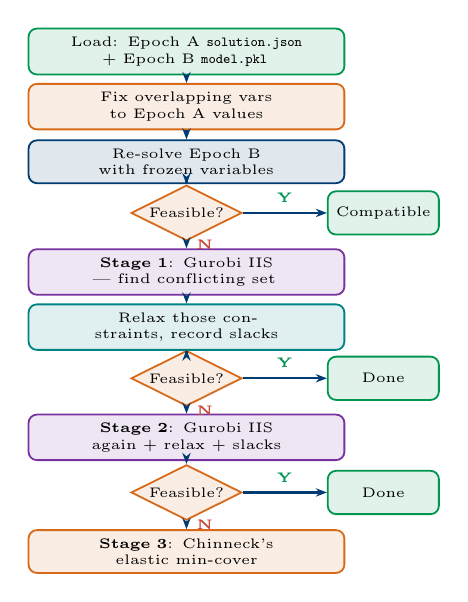
\begin{tikzpicture}
      \node[DB=3.8cm,minimum height=0.42cm,font=\tiny] at (0,5.6) (inp)
            {Load: Epoch A \texttt{solution.json}
             + Epoch B \texttt{model.pkl}};
      \node[PB=3.8cm,minimum height=0.42cm,font=\tiny] at (0,4.9) (fix)
            {Fix overlapping vars to Epoch A values};
      \draw[Arr] (inp)--(fix);
      \node[AB=3.8cm,minimum height=0.42cm,font=\tiny] at (0,4.2) (solve)
            {Re-solve Epoch B with frozen variables};
      \draw[Arr] (fix)--(solve);
      \node[DC,font=\tiny] at (0,3.55) (feas) {Feasible?};
      \draw[Arr] (solve)--(feas);
      \node[DB=1.2cm,font=\tiny] at (2.5,3.55) (ok)
            {Compatible \checkmark};
      \draw[Arr] (feas.east) --
            node[above,font=\tiny,text=lgrn]{\textbf{Y}} (ok.west);
      \node[RB=3.8cm,minimum height=0.42cm,font=\tiny] at (0,2.8) (iis)
            {\textbf{Stage 1}: Gurobi IIS — find conflicting set};
      \draw[Arr] (feas.south) --
            node[right,font=\tiny,text=ared]{\textbf{N}} (iis.north);
      \node[TB=3.8cm,minimum height=0.42cm,font=\tiny] at (0,2.1) (slack)
            {Relax those constraints, record slacks};
      \draw[Arr] (iis)--(slack);
      \node[DC,font=\tiny] at (0,1.45) (feas2) {Feasible?};
      \draw[Arr] (slack)--(feas2);
      \node[DB=1.2cm,font=\tiny] at (2.5,1.45) (done)
            {Done};
      \draw[Arr] (feas2.east) --
            node[above,font=\tiny,text=lgrn]{\textbf{Y}} (done.west);
      \node[RB=3.8cm,minimum height=0.42cm,font=\tiny] at (0,0.7) (iis2)
            {\textbf{Stage 2}: Gurobi IIS again + relax + slacks};
      \draw[Arr] (feas2.south) --
            node[right,font=\tiny,text=ared]{\textbf{N}} (iis2.north);
      \node[DC,font=\tiny] at (0,0.0) (feas3) {Feasible?};
      \draw[Arr] (iis2)--(feas3);
      \node[DB=1.2cm,font=\tiny] at (2.5,0.0) (done2)
            {Done};
      \draw[Arr] (feas3.east) --
            node[above,font=\tiny,text=lgrn]{\textbf{Y}} (done2.west);
      \node[PB=3.8cm,minimum height=0.42cm,font=\tiny] at (0,-0.75) (chinneck)
            {\textbf{Stage 3}: Chinneck's elastic min-cover};
      \draw[Arr] (feas3.south) --
            node[right,font=\tiny,text=ared]{\textbf{N}} (chinneck.north);
    \end{tikzpicture}
    \end{center}
  \end{column}
  \begin{column}{0.52\textwidth}
    \vspace{2pt}
    \begin{block}{Hybrid 3-stage approach}
      \small
      \begin{enumerate}\setlength\itemsep{2pt}
        \item \textbf{Gurobi IIS} — extract one minimal
              conflicting set. Relax those constraints,
              record slack values.
        \item \textbf{Re-check.} If still infeasible,
              Gurobi IIS again — second batch of
              blockers + slacks.
        \item \textbf{Chinneck's heuristic} — if
              \emph{still} infeasible, fall back to
              the elastic-constraints algorithm that
              identifies \emph{all} remaining violating
              constraints with minimum slacks.
      \end{enumerate}
    \end{block}
    \vspace{3pt}
    \begin{block}{Why hybrid?}
      \small Gurobi IIS is fast but finds only \emph{one}
      conflicting set per call. Chinneck's algorithm
      \textbf{guarantees the complete set} but is more
      expensive. The hybrid escalates only when needed —
      most models resolve in stage 1 or 2.
    \end{block}
    \vspace{3pt}
    \textcolor{mgray}{\scriptsize
      Output: every blocking constraint + its min slack to restore feasibility.}
  \end{column}
\end{columns}
\end{frame}

% ── QT3 JSON EXAMPLE ─────────────────────────────────────────
\begin{frame}[t]{QT3 JSON — \texttt{get\_comparison\_json("qt3")} Return Value}
\vspace{1pt}
\begin{block}{}
  \texttt{\scriptsize
    \{\,"qt": "QT3",\\
    \quad "epoch\_a": "q1\_supply\_abc",\\
    \quad "epoch\_b": "q2\_supply\_def",\\[1pt]
    \quad "summary": \{\\
    \quad\quad "compatible": false,\hfill\textcolor{ared}{\tiny verdict — Epoch A plan is infeasible in Epoch B}\\[1pt]
    \quad\quad "blocking\_constraints": [\hfill\textcolor{pblue}{\tiny all violating constraints found by hybrid approach}\\
    \quad\quad\quad "cap[Chicago]",\hfill\textcolor{pblue}{\tiny found in stage 1 (Gurobi IIS)}\\
    \quad\quad\quad "balance[Denver]"\hfill\textcolor{pblue}{\tiny found in stage 2 (second IIS round)}\\
    \quad\quad ],\\[1pt]
    \quad\quad "min\_relaxation": \{\hfill\textcolor{teal}{\tiny minimum RHS change to restore feasibility}\\
    \quad\quad\quad "cap[Chicago]": 26.0,\hfill\textcolor{teal}{\tiny relax capacity by 26 units}\\
    \quad\quad\quad "balance[Denver]": 14.5\hfill\textcolor{teal}{\tiny relax balance by 14.5 units}\\
    \quad\quad \}\\
    \quad \},\\[1pt]
    \quad "items": [\hfill\textcolor{mgray}{\tiny one entry per blocking constraint}\\
    \quad\quad \{\\
    \quad\quad\quad "constraint": "cap[Chicago]",\hfill\textcolor{mgray}{\tiny which constraint blocks}\\
    \quad\quad\quad "slack\_needed": 26.0,\hfill\textcolor{teal}{\tiny min relaxation to make this constraint feasible}\\
    \quad\quad\quad "stage": 1\hfill\textcolor{aorng}{\tiny discovered in Gurobi IIS round 1}\\
    \quad\quad \},\\
    \quad\quad \ldots\quad\textcolor{mgray}{// one entry per blocker — all constraints accounted for}\\
    \quad ],\\
    \quad "truncated": false,\hfill\textcolor{lgrn}{\tiny all blockers shown — nothing hidden}\\
    \quad "total\_count": 2\hfill\textcolor{lgrn}{\tiny only 2 blocking constraints found}\\
    \}
  }
\end{block}
\vspace{1pt}
\centering\scriptsize
\textcolor{ared}{$\blacksquare$}\,Feasibility verdict\quad
\textcolor{pblue}{$\blacksquare$}\,Blocking constraints\quad
\textcolor{teal}{$\blacksquare$}\,Slack values\quad
\textcolor{aorng}{$\blacksquare$}\,Discovery stage\quad
\textcolor{lgrn}{$\blacksquare$}\,Complete result\qquad
\textcolor{mgray}{\textit{Hybrid: Gurobi IIS (×2) $\to$ Chinneck's heuristic if needed.}}
\end{frame}

% ── SLIDE 15a · QT4 — ALGORITHM ────────────────────────────────
\begin{frame}[t]{QT4 — Solution Attribution: Why Did the Solution Change?}
\vspace{2pt}
\begin{columns}[T]
  \begin{column}{0.50\textwidth}
    \small\textbf{User asks:}
    \emph{``Why did the solution change between epochs?
    What drove the shift in optimal decisions?''}
    \vspace{5pt}
    \textbf{Algorithm — Parameters $\to$ Constraints $\to$ Variables:}
    \begin{enumerate}\setlength\itemsep{3pt}
      \item \textbf{Get LP duals} from both epochs — for
            every constraint.
            LP: read from \texttt{solution.json}.
            MIP: re-solve LP relaxation, cache to
            \texttt{duals.json}.
      \item \textbf{Bottleneck evolution} — compare each
            constraint's dual across epochs. Classify as
            \emph{relieved}, \emph{new bottleneck}, or
            \emph{persistent}. Keep \textbf{top N} by
            dual magnitude.
      \item For each top constraint, look up
            (from \texttt{structure.json}):
            \begin{itemize}\setlength\itemsep{1pt}
              \item[\textcolor{aorng}{$\uparrow$}]
                    \textbf{Parameters} that feed into it
                    — which of them shifted? (from QT1)
              \item[\textcolor{purp}{$\downarrow$}]
                    \textbf{Variables} that participate in it
                    — binary flips + continuous changes
                    (top 3 per constraint)
            \end{itemize}
      \item \textbf{Narrative} — code assembles a
            5-field story; the LLM does not write it.
    \end{enumerate}
  \end{column}
  \begin{column}{0.46\textwidth}
    \begin{block}{Bottleneck evolution}
      \small
      Every constraint has a \textbf{dual value} that
      tells you how sensitive the objective is to it.
      Comparing duals across epochs reveals:\\[4pt]
      \textcolor{lgrn}{\textbf{Relieved}}: binding in A, relaxed in B
      — stopped being a bottleneck.\\[3pt]
      \textcolor{ared}{\textbf{New bottleneck}}: relaxed in A, binding in B
      — became a bottleneck.\\[3pt]
      \textcolor{aorng}{\textbf{Persistent}}: binding in both
      — sensitivity may have shifted.
    \end{block}
    \vspace{5pt}
    \begin{block}{Each constraint carries context in both directions}
      \small
      \textcolor{aorng}{$\uparrow$\,\textbf{Up}}: which parameters
      (QT1) feed into this constraint and changed?
      \emph{Why it shifted.}\\[3pt]
      \textcolor{purp}{$\downarrow$\,\textbf{Down}}: which variables
      in this constraint changed?
      \emph{What decisions were affected.}\\[3pt]
      One cap at the constraint level controls the
      entire output size.
    \end{block}
  \end{column}
\end{columns}
\end{frame}

% ── SLIDE 15b · QT4 — NARRATIVE ──────────────────────────────
\begin{frame}[t]{QT4 — From Constraints to Narrative}
\vspace{2pt}
\begin{columns}[T]
  \begin{column}{0.50\textwidth}
    \begin{exampleblock}{Example — one constraint, full story}
      \small
      \texttt{cap[Denver]} became a \textbf{new bottleneck}
      (dual 0 $\to$ 1.4).\\[4pt]
      \textcolor{aorng}{$\uparrow$ \textbf{Why?}} \texttt{demand[Denver]}
      rose 22\% (from QT1).\\[4pt]
      \textcolor{purp}{$\downarrow$ \textbf{What changed?}}
      \texttt{use\_warehouse[Denver]} flipped 0$\to$1.
      \texttt{assign[Denver]} rose 40\%.\\[4pt]
      $\Rightarrow$ \emph{``Denver demand rose 22\%,
      the capacity constraint tightened, the warehouse
      activated and allocation increased.''}\\[4pt]
      \textcolor{mgray}{\scriptsize One constraint entry = one paragraph
      of the answer.}
    \end{exampleblock}
    \vspace{4pt}
    \begin{block}{Why cap at constraints?}
      \small
      Constraints sit in the middle of the hierarchy.
      Capping top N constraints automatically limits both
      the parameter context above and the variable detail
      below. One knob controls the full output size.
    \end{block}
  \end{column}
  \begin{column}{0.46\textwidth}
    \begin{block}{The 5-field narrative — built by code}
      \small The LLM receives this pre-written and uses it
      as the backbone of its answer.
      \vspace{4pt}
      \renewcommand{\arraystretch}{1.4}
      \scriptsize
      \begin{tabular}{@{}p{2.3cm}@{\ }p{3.8cm}@{}}
        \toprule
        \textbf{Field} & \textbf{Source} \\
        \midrule
        \textbf{parameter\_shift} & \textcolor{aorng}{$\uparrow$ QT1}: which
                                    inputs changed \\
        \textbf{prior\_state}     & \textcolor{ared}{Duals A}: constraints
                                    binding before \\
        \textbf{adaptation}       & \textcolor{purp}{$\downarrow$ Variables}:
                                    flips + continuous shifts \\
        \textbf{outcome}          & \textcolor{teal}{QT2}: net effect on
                                    objective \\
        \textbf{new\_state}       & \textcolor{ared}{Duals B}: constraints
                                    binding now \\
        \bottomrule
      \end{tabular}
    \end{block}
    \vspace{4pt}
    \textcolor{mgray}{\scriptsize\textit{Associative language — ``associated
    with,'' not ``caused by.''}}
  \end{column}
\end{columns}
\end{frame}

% ── QT4 JSON EXAMPLE ─────────────────────────────────────────
\begin{frame}[t]{QT4 JSON — \texttt{get\_comparison\_json("qt4")} Return Value}
\vspace{1pt}
\begin{block}{}
  \texttt{\scriptsize
    \{\,"qt": "QT4",\\
    \quad "epoch\_a": "q1\_supply\_abc",\\
    \quad "epoch\_b": "q2\_supply\_def",\\[2pt]
    \quad "bottleneck\_evolution": [\hfill\textcolor{mgray}{\tiny top N constraints by dual shift}\\[1pt]
    \quad\quad \{"constraint": "cap[Denver]",\\
    \quad\quad\quad "dual\_a": 0.0,\ "dual\_b": 1.4,\\
    \quad\quad\quad "status": "new\_bottleneck",\hfill\textcolor{ared}{\tiny became binding in Epoch B}\\[2pt]
    \quad\quad\quad "param\_shifts": [\hfill\textcolor{aorng}{\tiny $\uparrow$ which inputs in this constraint changed}\\
    \quad\quad\quad\quad \{"param": "demand[Denver]",\ "delta": 0.22\}\\
    \quad\quad\quad ],\\[2pt]
    \quad\quad\quad "variables": [\hfill\textcolor{purp}{\tiny $\downarrow$ which decisions in this constraint changed}\\
    \quad\quad\quad\quad \{"var": "use\_wh[Den]",\ "type": "binary",\ "flip": "0$\to$1"\},\\
    \quad\quad\quad\quad \{"var": "assign[Den]",\ "type": "continuous",\\
    \quad\quad\quad\quad\quad "val\_a": 80,\ "val\_b": 112,\ "delta": 0.40\}\\
    \quad\quad\quad ]\\
    \quad\quad \},\\
    \quad\quad \ldots\quad\textcolor{mgray}{// more constraints (relieved, persistent)}\\
    \quad ],\\[3pt]
    \quad "narrative": \{\hfill\textcolor{pblue}{\tiny pre-written story — agent uses verbatim}\\
    \quad\quad "parameter\_shift": "demand[Denver] rose 22\%",\\
    \quad\quad "prior\_state":\ \ \ "cap[Denver] was not binding",\\
    \quad\quad "adaptation":\ \ \ \ "warehouse activated, allocation +40\%",\\
    \quad\quad "outcome":\ \ \ \ \ \ "cost increased 2.6\%",\\
    \quad\quad "new\_state":\ \ \ \ "cap[Denver] now binding (dual 1.4)"\\
    \quad \}\\
    \}
  }
\end{block}
\vspace{1pt}
\centering\scriptsize
\textcolor{ared}{$\blacksquare$}\,Bottleneck shift\quad
\textcolor{purp}{$\blacksquare$}\,Variable attribution\quad
\textcolor{aorng}{$\blacksquare$}\,Parameter shifts\quad
\textcolor{pblue}{$\blacksquare$}\,Narrative\qquad
\textcolor{mgray}{\textit{Constraints $\to$ variables $\to$ story. Code-built, non-causal.}}
\end{frame}

% ── SLIDE 17 · SUMMARY 1 ───────────────────────────────────────
\begin{frame}{Summary — Architecture \& Intelligence}
\begin{columns}[T]
  \begin{column}{0.48\textwidth}
    \begin{block}{Architecture}
      \begin{itemize}\setlength\itemsep{4pt}
        \item Two-agent hierarchy: root classifies,
              comparison agent executes — clear responsibility split
        \item Prompt rebuilt before every LLM call — no stale state
        \item Isolated ADK app with independent session namespace
      \end{itemize}
    \end{block}
  \end{column}
  \begin{column}{0.48\textwidth}
    \begin{block}{Intelligence}
      \begin{itemize}\setlength\itemsep{4pt}
        \item LLM-based classification: robust to phrasing,
              no keyword maintenance
        \item Two-step NL resolution: discover families first,
              then match semantically — works across any naming convention
      \end{itemize}
    \end{block}
  \end{column}
\end{columns}
\end{frame}
% ── SLIDE 18 · SUMMARY 2 ───────────────────────────────────────
\begin{frame}{Summary — Data, Caching \& Scale}
\begin{columns}[T]
  \begin{column}{0.48\textwidth}
    \begin{block}{Data and Caching}
      \begin{itemize}\setlength\itemsep{4pt}
        \item Two-level cache (disk + in-process): same epoch pair
              never reanalysed
        \item Uniform QT JSON schema: one structure for all four
              modules — simpler agent code
      \end{itemize}
    \end{block}
  \end{column}
  \begin{column}{0.48\textwidth}
    \begin{block}{Scale}
      \begin{itemize}\setlength\itemsep{4pt}
        \item Hard token caps prevent context overflow on
              large enterprise models
        \item Lazy loading: \texttt{model.pkl} never touched
              unless a solver is actually needed
        \item Progressive disclosure: summary $\to$ drill-down
              $\to$ raw file — exactly as much detail as requested
      \end{itemize}
    \end{block}
  \end{column}
\end{columns}
\end{frame}
% ============================================================
%  EXAMPLE SLIDES — Pricing & Promotion Placement Model
% ============================================================

% --- Slide: Data Comparison ---------------------------------
\begin{frame}[t]{Example — Pricing \& Promotion Placement Model}
\vspace{1pt}
\centering{\small\textit{Optimise promotional vehicle placements across periods
to maximise profit-weighted exposure, subject to slot and budget constraints.}}
\vspace{4pt}
\begin{columns}[T]
  \begin{column}{0.46\textwidth}
    \begin{block}{\scriptsize Epoch A}
      \scriptsize
      \renewcommand{\arraystretch}{1.15}
      \begin{tabular}{@{}l@{\;\;}l@{}}
        \textbf{Horizon}       & 10 periods \\
        \textbf{Vehicles}      & Front, Endcap, TV, \\
                                & Aisle, Checkout \\
        \textbf{Slot cap.}     & 3 / period \\
        \textbf{$\varepsilon$} & 0.05 \\
        \textbf{Profit wt.}    & \$300 (uniform) \\
        \textbf{Budgets}       & Fr\,5\; End\,6\; TV\,6 \\
                                & Ais\,5\; Chk\,7 \\
        \textbf{Boosts}        & Fr\,1.35\; End\,1.25 \\
                                & TV\,1.15\; Ais\,1.18 \\
                                & Chk\,1.12 \\
      \end{tabular}
    \end{block}
  \end{column}
  \begin{column}{0.50\textwidth}
    \begin{block}{\scriptsize Epoch B \quad\textcolor{ared}{\scriptsize$\blacktriangle$ = changed}}
      \scriptsize
      \renewcommand{\arraystretch}{1.15}
      \begin{tabular}{@{}l@{\;\;}l@{}}
        \textbf{Horizon}       & \textcolor{ared}{12} periods \textcolor{ared}{\scriptsize(+2)} \\
        \textbf{Vehicles}      & Front, Endcap, TV, Aisle, \\
                                & Checkout, \textcolor{ared}{Social} \\
        \textbf{Slot cap.}     & \textcolor{ared}{2} / period \textcolor{ared}{\scriptsize($\downarrow$)} \\
        \textbf{$\varepsilon$} & \textcolor{ared}{0.03} \textcolor{ared}{\scriptsize($\downarrow$)} \\
        \textbf{Profit wt.}    & \textcolor{ared}{\$400--\$600 (seasonal)} \\
        \textbf{Budgets}       & Fr\,\textcolor{ared}{3}\; End\,\textcolor{ared}{4}\; TV\,\textcolor{ared}{4} \\
                                & Ais\,\textcolor{ared}{4}\; Chk\,\textcolor{ared}{5}\; \textcolor{ared}{Soc\,6} \\
        \textbf{Boosts}        & Fr\,\textcolor{ared}{1.50}\; End\,\textcolor{ared}{1.30} \\
                                & TV\,\textcolor{ared}{1.20}\; Ais\,\textcolor{ared}{1.20} \\
                                & Chk\,\textcolor{ared}{1.10}\; \textcolor{ared}{Soc\,1.40} \\
      \end{tabular}
    \end{block}
  \end{column}
\end{columns}
\vspace{4pt}
\centering\scriptsize
\textcolor{ared}{\textbf{Key shifts:}}
Horizon extended $\cdot$ New vehicle type $\cdot$ Slot capacity halved $\cdot$
Budgets tightened $\cdot$ Weights now seasonal $\cdot$ Boosts generally increased
\end{frame}

% --- Q\&A Slide 1: Structural Changes (QT1) ----------------
\begin{frame}[t]{Example — QT1: Structural Comparison}
\vspace{2pt}

\begin{tikzpicture}
  \node[fill=lblue, rounded corners=3pt, text width=14.2cm,
        inner xsep=8pt, inner ysep=5pt] {
    \small\textbf{\textcolor{pblue}{Q:}}\;
    \textit{Are there any structural changes between the two model instances?}
  };
\end{tikzpicture}
\vspace{6pt}
\small\textbf{\textcolor{lgrn}{A:}}\;
Yes --- two structural changes were detected between Epoch\,A and Epoch\,B:
\vspace{2pt}
\begin{itemize}\setlength\itemsep{5pt}
  \item \textbf{Planning horizon extended:} 10 periods $\to$ 12 periods
        \textcolor{mgray}{(periods 11 and 12 added)}
  \item \textbf{New vehicle type:} ``Social'' added to the vehicle set
        \textcolor{mgray}{(5 $\to$ 6 vehicles)}
  \item The mathematical structure (constraint types, objective form) is
        \textbf{unchanged} --- same model template, expanded index sets
\end{itemize}
\vspace{6pt}

\begin{tikzpicture}
  \node[fill=lgray, rounded corners=3pt, text width=14.2cm,
        inner xsep=8pt, inner ysep=4pt] {
    \scriptsize\textcolor{mgray}{\textbf{Takeaway:}\;
    The model grew in size (new variables and constraints for added indices)
    but the underlying formulation logic did not change.}
  };
\end{tikzpicture}
\end{frame}

% --- Q\&A Slide 2: Input Data Changes (QT1) ----------------
\begin{frame}[t]{Example — QT1: Input Data Changes}
\vspace{2pt}

\begin{tikzpicture}
  \node[fill=lblue, rounded corners=3pt, text width=14.2cm,
        inner xsep=8pt, inner ysep=5pt] {
    \small\textbf{\textcolor{pblue}{Q:}}\;
    \textit{What changed in the input data between the two solves?}
  };
\end{tikzpicture}
\vspace{4pt}
\small\textbf{\textcolor{lgrn}{A:}}\;
Several parameter shifts were identified across both epochs:
\vspace{2pt}
\footnotesize
\begin{itemize}\setlength\itemsep{3pt}
  \item \textbf{Slot capacity reduced:} 3 $\to$ 2 vehicles per period
        \textcolor{mgray}{(33\% fewer placements per slot)}
  \item \textbf{Usage budgets tightened:} all existing vehicles received lower caps
        \textcolor{mgray}{(e.g.\ Front 5$\to$3, Checkout 7$\to$5)}
  \item \textbf{Profit weights:} flat \$300 $\to$ seasonal \$400\,--\,\$600
        \textcolor{mgray}{(peaks in periods 4--6 and 12)}
  \item \textbf{Boosts increased:} Front 1.35$\to$1.50,\; Endcap 1.25$\to$1.30,\;
        TV 1.15$\to$1.20
  \item \textbf{Epsilon tightened:} 0.05 $\to$ 0.03
        \textcolor{mgray}{(stricter balance requirement)}
\end{itemize}
\vspace{4pt}
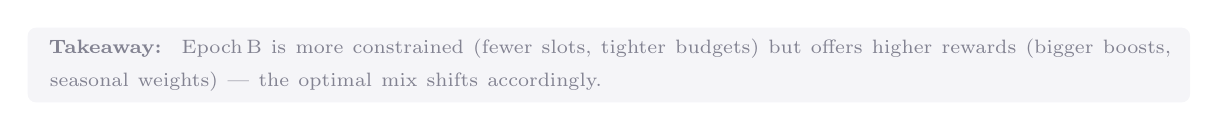
\begin{tikzpicture}
  \node[fill=lgray, rounded corners=3pt, text width=14.2cm,
        inner xsep=8pt, inner ysep=4pt] {
    \scriptsize\textcolor{mgray}{\textbf{Takeaway:}\;
    Epoch\,B is more constrained (fewer slots, tighter budgets) but offers higher
    rewards (bigger boosts, seasonal weights) --- the optimal mix shifts accordingly.}
  };
\end{tikzpicture}
\end{frame}

% --- Q\&A Slide 3: Solution Changes (QT2) ------------------
\begin{frame}[t]{Example — QT2: Solution Comparison}
\vspace{2pt}

\begin{tikzpicture}
  \node[fill=lblue, rounded corners=3pt, text width=14.2cm,
        inner xsep=8pt, inner ysep=5pt] {
    \small\textbf{\textcolor{pblue}{Q:}}\;
    \textit{How did the optimal solution change between the two solves?}
  };
\end{tikzpicture}
\vspace{4pt}
\small\textbf{\textcolor{lgrn}{A:}}\;
The solution shifted significantly due to combined structural and parametric changes:
\vspace{2pt}
\footnotesize
\begin{itemize}\setlength\itemsep{3pt}
  \item \textbf{Objective value increased} --- higher profit weights and boosts
        more than offset the tighter capacity constraints
  \item \textbf{Total active placements reduced:} 29 $\to$ 24
        \textcolor{mgray}{(slot capacity 3$\to$2 is now the binding constraint)}
  \item \textbf{Allocation shift:} high-boost vehicles (Front\,1.50, Social\,1.40)
        gained priority over lower-boost vehicles (Checkout, Aisle)
  \item \textbf{Temporal concentration:} placements now cluster in high-profit
        periods (4--6, 10--12) rather than spreading uniformly
\end{itemize}
\vspace{4pt}
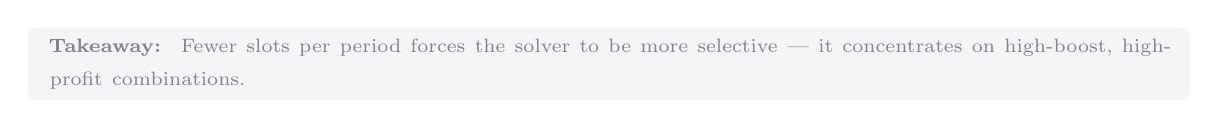
\begin{tikzpicture}
  \node[fill=lgray, rounded corners=3pt, text width=14.2cm,
        inner xsep=8pt, inner ysep=4pt] {
    \scriptsize\textcolor{mgray}{\textbf{Takeaway:}\;
    Fewer slots per period forces the solver to be more selective ---
    it concentrates on high-boost, high-profit combinations.}
  };
\end{tikzpicture}
\end{frame}

% --- Q\&A Slide 4: Per-Vehicle Breakdown (QT2 drill-down) --
\begin{frame}[t]{Example — QT2: Per-Vehicle Allotment Shifts}
\vspace{2pt}

\begin{tikzpicture}
  \node[fill=lblue, rounded corners=3pt, text width=14.2cm,
        inner xsep=8pt, inner ysep=5pt] {
    \small\textbf{\textcolor{pblue}{Q:}}\;
    \textit{How did the allotments shift for each vehicle type across the two solves?}
  };
\end{tikzpicture}
\vspace{4pt}
\small\textbf{\textcolor{lgrn}{A:}}\;Per-vehicle allocation comparison:
\vspace{3pt}
\centering\footnotesize
\renewcommand{\arraystretch}{1.25}
\begin{tabular}{@{} l c c c c l @{}}
\toprule
\textbf{Vehicle} & \textbf{Ep.\,A} & \textbf{Ep.\,B} & \textbf{$\Delta$} & \textbf{Boost} & \textbf{Notes} \\
\midrule
Front    & 5  & 3  & $-$2 & 1.35$\to$1.50 & Budget-limited; highest boost \\
Endcap   & 6  & 4  & $-$2 & 1.25$\to$1.30 & Budget now binding \\
TV       & 6  & 4  & $-$2 & 1.15$\to$1.20 & Displaced by Social \\
Aisle    & 5  & 4  & $-$1 & 1.18$\to$1.20 & Lower priority \\
Checkout & 7  & 3  & $-$4 & 1.12$\to$1.10 & Lowest boost; biggest drop \\
Social   & -- & 6  & \textcolor{lgrn}{+6} & \textcolor{lgrn}{new\,1.40} & New entrant; 2nd highest boost \\
\midrule
\textbf{Total} & \textbf{29} & \textbf{24} & $-$5 & & Slot cap now binding \\
\bottomrule
\end{tabular}
\vspace{4pt}
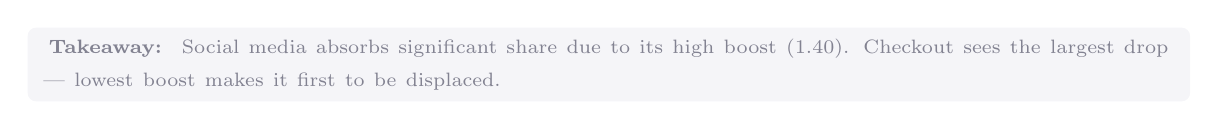
\begin{tikzpicture}
  \node[fill=lgray, rounded corners=3pt, text width=14.2cm,
        inner xsep=8pt, inner ysep=4pt] {
    \scriptsize\textcolor{mgray}{\textbf{Takeaway:}\;
    Social media absorbs significant share due to its high boost (1.40).
    Checkout sees the largest drop --- lowest boost makes it first to be displaced.}
  };
\end{tikzpicture}
\end{frame}

% --- Q\&A Slide 5: Backward Compatibility (QT3) ------------
\begin{frame}[t]{Example — QT3: Backward Compatibility}
\vspace{2pt}

\begin{tikzpicture}
  \node[fill=lblue, rounded corners=3pt, text width=14.2cm,
        inner xsep=8pt, inner ysep=5pt] {
    \small\textbf{\textcolor{pblue}{Q:}}\;
    \textit{Can the previous vehicle allotment plan still be used under the current inputs?}
  };
\end{tikzpicture}
\vspace{6pt}
\small\textbf{\textcolor{lgrn}{A:}}\;
\textbf{No} --- the previous allotment cannot be used as-is.
\vspace{2pt}
\begin{itemize}\setlength\itemsep{5pt}
  \item The old plan assigned \textbf{Front} to \textbf{5 periods},
        but Epoch\,B's usage budget only allows \textbf{3}
  \item This violates the tightened Front vehicle usage budget constraint
  \item To restore feasibility, either:
        \begin{itemize}\setlength\itemsep{2pt}
          \item Increase the Front budget back toward its old level, or
          \item Reduce Front assignments in the old plan to fit the new cap
        \end{itemize}
\end{itemize}
\end{frame}

% --- Q\&A Slide 6: Feasibility Restoration (QT3 follow-up) -
\begin{frame}[t]{Example — QT3: Feasibility Restoration}
\vspace{2pt}

\begin{tikzpicture}
  \node[fill=lblue, rounded corners=3pt, text width=14.2cm,
        inner xsep=8pt, inner ysep=5pt] {
    \small\textbf{\textcolor{pblue}{Q:}}\;
    \textit{By how much should the Front budget be increased to reuse the previous allotment plan?}
  };
\end{tikzpicture}
\vspace{6pt}
\small\textbf{\textcolor{lgrn}{A:}}\;
Increase the Front budget by \textbf{2} (from 3 back up to 5).
\vspace{2pt}
\begin{itemize}\setlength\itemsep{5pt}
  \item This restores the capacity \texttt{C[Front]\,=\,5} used in Epoch\,A
  \item Makes the earlier vehicle allotment plan fully feasible under Epoch\,B's rules
  \item \textcolor{mgray}{\textit{Alternative:}} increase to 4 and reassign a few
        placements to other vehicles --- achieves similar coverage with a smaller
        budget change
\end{itemize}
\end{frame}

% --- Q\&A Slide 7: Solution Attribution (QT4) --------------
\begin{frame}[t]{Example — QT4: Why Did the Allotment Plan Change?}
\vspace{2pt}

\begin{tikzpicture}
  \node[fill=lblue, rounded corners=3pt, text width=14.2cm,
        inner xsep=8pt, inner ysep=5pt] {
    \small\textbf{\textcolor{pblue}{Q:}}\;
    \textit{Why did my allotment plan change between the two solves?}
  };
\end{tikzpicture}
\vspace{4pt}
\small\textbf{\textcolor{lgrn}{A:}}\;
Two main drivers caused the plan to shift:
\vspace{2pt}
\footnotesize
\begin{itemize}\setlength\itemsep{3pt}
  \item \textbf{Increased period weights:} Periods 4--6 and 10 gained higher profit
        weights, making those windows more attractive for placements
  \item \textbf{Tighter Front budget:} Front's allowed uses were cut (5$\to$3),
        so remaining Front placements concentrated into the highest-return periods
        and lower-value placements were dropped
  \item \textbf{Net effect:} Fewer total placements but better-targeted ones ---
        assignments moved into higher-impact periods and locations
\end{itemize}
\vspace{6pt}
\small\textbf{Actions you can take:}
\footnotesize
\begin{itemize}\setlength\itemsep{3pt}
  \item If the new priorities are intentional, accept the change
  \item To restore prior coverage: increase Front budget (+2) or
        substitute other vehicles in the dropped slots
\end{itemize}
\end{frame}
\end{document}
